\documentclass[12pt,a4paper]{article}

\usepackage[utf8]{inputenc}
\usepackage[T1]{fontenc}
\usepackage[french]{babel}

\usepackage{amsmath, amssymb}

\usepackage{graphicx}
\usepackage{caption}

\usepackage{siunitx} % Pour les unités

\usepackage{geometry}
\geometry{top=2cm, bottom=2.5cm, left=3cm, right=3cm}
\setlength{\parindent}{0pt}


\usepackage{enumitem}

\usepackage{hyperref}

\usepackage{xcolor}

\usepackage{multicol}
\setlength{\columnseprule}{1pt}
\def\columnseprulecolor{\color{gray}}

\usepackage{tcolorbox}


\usepackage{import}
\usepackage{xifthen}
\usepackage{pdfpages}
\usepackage{transparent}
\usepackage{float}

\newcommand{\incfig}[1]{%
	\def\svgwidth{\columnwidth}
	\import{./figures/}{#1.pdf_tex}
}


\newcommand{\RomanNum}[1] %pour les chiffre romain
{\MakeUppercase{\romannumeral #1}}



\usepackage{wrapfig}







\title{|}
\author{}
\date{\today}

\begin{document}
	\counterwithin{section}{part} % pour que \section{} recommence de 1 aprés \part{}
	
	
	\tableofcontents
	
	\newpage
	
	
	
	\part{Rappels}
	
	
	
	\section{Écriture de la contrainte}
	
	La contrainte représente une pression sur une surface donnée uniforme ou non du au systéme d'action appliquer a notre section.
	
	
	\section{La compression simple}
	
	\[ N \neq 0 \quad;\quad M = 0 \]
	
	Avec la convetion de signe $N > 0$
	
	\vspace{\baselineskip}
	
	La contrainte est écrite ainsi :
	
	\[ \sigma = \dfrac{N}{S} \]
	
	\section{Traction simple}
	
	\[ N \neq 0 \quad;\quad M = 0 \]
	
	Avec la convetion de signe $N < 0$
	
	\[ \sigma = \dfrac{N}{S} \]
	
	
	
	\section{Flexion simple}
	
	\[ N = 0 \quad;\quad M \neq 0 \]
	
	Donc la contrainte a un point donnée $y$ est de : 
	
	\[ \sigma = \dfrac{M \cdot y}{I} \] 
	
	\begin{tcolorbox}[colback=gray!20, colframe=black, title=Remarque]
		
	L'effort dans la fibre comprimé = L'effot dans la fibre tendu.
	
	\end{tcolorbox}
	
	
	
	\begin{figure}[H]
		\centering
		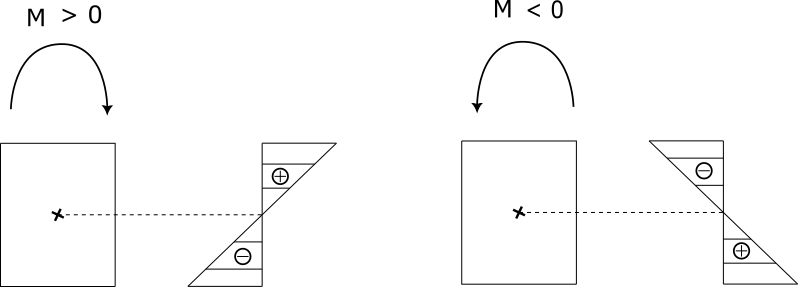
\includegraphics[width=0.7\linewidth]{figures/moment-+-}
		\label{fig:moment--}
	\end{figure}
	
	\vspace{5\baselineskip}

	\begin{figure}[H]
		\centering
		\begin{minipage}{0.5\textwidth}
			\raggedright
			\[ \sigma > 0 \quad\text{Zone comprimé} \]
		\end{minipage}%
		\hfill
		\begin{minipage}{0.5\textwidth}
			\centering
			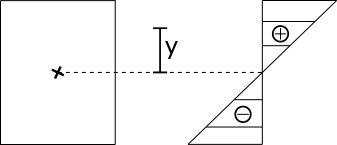
\includegraphics[width=0.7\linewidth]{figures/zone-comprime}
			\caption{Zone comprimé}
		\end{minipage}
	\end{figure}
	
	
	
	\begin{figure}[H]
		\centering
		\begin{minipage}{0.5\textwidth}
			\raggedright
			\[ \sigma < 0 \quad\text{Zone tendu} \]
		\end{minipage}%
		\hfill
		\begin{minipage}{0.5\textwidth}
			\centering
			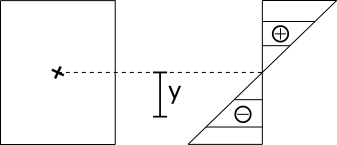
\includegraphics[width=0.7\linewidth]{figures/zone-tendu}
			\caption{Zone tendu}
		\end{minipage}
	\end{figure}
	
	
	
	
	\[ \sigma = 0 \quad \text{Zone neutre (axe neutre) } y=0  \]
	
	
	
	\begin{tcolorbox}[colback=gray!20, colframe=black, title=Remarque]
		On peut connaitre la contrainte a un point y quelconque.
		
		Donc si on cherche la contrainte a la fibre supérieur y = V et pour la fibre inferieur y = V' en sachant que V' est négatif.
	\end{tcolorbox}
	
	
	
	\section{Flexion composée}
	
	\[ N \neq 0 \quad;\quad M \neq 0 \]
	
	
	
	
	En quelconque point y de la section on aura : 
	
	\[ \sigma = \dfrac{N}{S} \pm \dfrac{M \cdot y}{I}  \]
	
	
	Que ca soit postitif ou négatif sela dépend de y.
	
	\begin{tcolorbox}[colback=gray!20, colframe=black, title=Remarque]
		On peut avoir une flexion composée si la force N appliquer sur la section est excentrée donc on transpose cette force vers le CDG puis on crée un moment $M = N \cdot e$ avec $e$ étant l'excentricité.
		
		\begin{figure}[H]
			\centering
			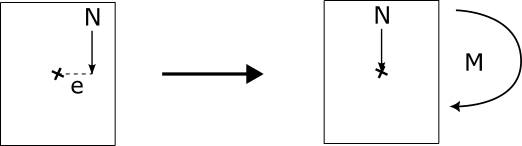
\includegraphics[width=0.7\linewidth]{figures/force-excentree}
			\label{fig:force-excentree}
		\end{figure}
		
		
	\end{tcolorbox}
	
	
	\section{Flexion déviée}
	
	\[ N = 0 \quad;\quad M_{x} \neq 0 \quad;\quad M_{y} \neq 0 \]
	
	$M_{y}$ : Moment flechissant autour de l'axe y.
	
	$M_{x}$ : Moment flechissant autor de l'axe x.
	
	La contrainte devient :
	
	\[ \sigma = \pm\dfrac{M_{x} \cdot y}{I_{x}} \pm\dfrac{M_{y} \cdot x}{I_{y}} \]
	
	Donc la contrainte est comme une superposition des contrainte selon x et selon y.
	
	
	
	
	\section{Flexion composée déviée (flexion composée oblique)}
	
	
	\[ N \neq 0 \quad;\quad M_{x} \neq 0 \quad;\quad M_{y} \neq 0 \]
	
	
	\[ \sigma = \dfrac{N}{S} \pm\dfrac{M_{x} \cdot y}{I_{x}} \pm\dfrac{M_{y} \cdot x}{I_{y}} \]
	
	
	\begin{tcolorbox}[colback=gray!20, colframe=black, title=Remarque]
		On peut aussi avoir ce cas uniquement en ayant une force exenctrée aussi
		
		\begin{figure}[H]
			\centering
			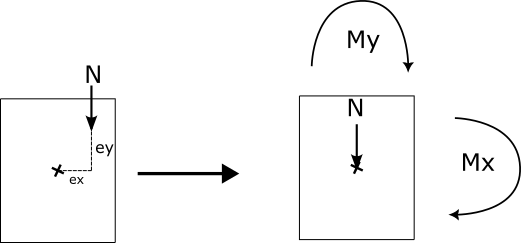
\includegraphics[width=0.7\linewidth]{figures/force-excentree2}
			\label{fig:force-excentree2}
		\end{figure}
		
	\end{tcolorbox}
	
	
	\section{Contrainte a la pre-contrainte}
	
	\[ \sigma_{p} = \dfrac{P}{S} \pm\dfrac{M_{p} \cdot y}{I} \]
	
	
	
	
	\begin{tcolorbox}[colback=gray!20, colframe=black, title=Remarque]
		On réalise les ponts en appuie simple pour éviter la transsmission des moments au piles.
	\end{tcolorbox}
	
	
	\part{title}
	
	\section{Les matériaux}
	
	
	
	\subsection{Le béton}
	
	
	\subsubsection{Résistance a la compression}
	
	La résistance a la compression doit etre $f_{c28} \geq 30~\unit{MPa}$ car une valeur en dessous le béton peut s'écraser avec la force de la pré-contrainte.
	
	\subsubsection{Résistance a la traction}
	
	\[ f_{t28} = 0,6 + 0,06 \cdot f_{c28} \]
	
	\subsubsection{Résistance a j jours}
	
	\[ f_{cj} = 0,685 \cdot \log(j+1) \cdot f_{c28} \]
	
	\subsubsection{Module de Young}
	
	\paragraph{Module instantané}
	
	\[ E_{i} = 11000 \cdot \sqrt[3]{f_{c28}} \]
	
	\paragraph{Module différé} 
	
	\[ E_{d} = 3700 \cdot \sqrt[3]{f_{c28}} \]
	
	
	\[ E_{d} < E_{i} \]
	
	
	\begin{tcolorbox}[colback=gray!20, colframe=black, title=Remarque]
		Le module instantané (ou module initial, module court terme) de Young est mesuré juste après l’application de la charge,
		avant que le matériau n’ait le temps de se déformer lentement (fluage).
		
		\vspace{\baselineskip}
		
		Le module différé de Young apparent quand la charge agit pendant longtemps — il tient compte du fluage (déformation lente sous contrainte constante).
		
		\vspace{2\baselineskip}
		
		Le module chute a long terme a cause du fluage.
		
		\vspace{\baselineskip}
		
		Le module instantané est utiliser pour les calculs a court terme et le différé pour les calculs a long terme.
		
	\end{tcolorbox}
	
	
	\subsection{Déformations du béton}
	
	Si on prends pas en compte les déformations du béton a la précontrainte les cables du précontainte risque de perdre en tension, car le béton se déforme lentement et les cables suivent cette déformation, et cela peut causer des fissures ou bien l'ouverture des fissures (cas fissures non pré-judicable), une fléche excessive a long terme et aussi un déséquilibre.
	

	\subsubsection{Le retrait du béton}
	
	C'est un phénomene du a l'évaporation de l'eau dans le béton générant un raccoursissement du béton.
	
	\subsubsection{Le fluage du béton}
	
	\begin{minipage}{0.6\textwidth}
		
		C'est une déformation qui apparait dans des piéces en béton soumise a un 
		effort de compression maintenue constament dans le temps.
	
	\end{minipage}
	\begin{minipage}{0.4\textwidth}
		
		\begin{figure}[H]
			\centering
			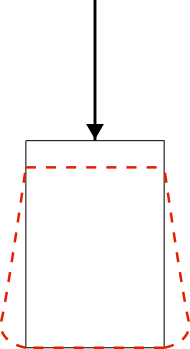
\includegraphics[width=0.3\linewidth]{figures/fluage}
			\label{fig:fluage}
		\end{figure}
		
	
	\end{minipage}
	
	
	
	
	\subsection{Les armatures}
	
	\subsubsection{Les barres d'aciers}
	
	\[ \phi > 12~\unit{mm} \]
	
	\subsubsection{Les fils de précontainte}
	
	\[ \phi < 12~\unit{mm} \]
	
	\subsubsection{Les torons}
	
	\begin{minipage}{0.7\textwidth}
		
		C'est un ensemble de fils enroulée autour d'un fil centrale le plus utilisé est 7 fils, le diamétre du toron de $13~\unit{mm}$ (plus utilisé) (T13)
		
	\end{minipage}
	\begin{minipage}{0.3\textwidth}
		
		\begin{figure}[H]
			\centering
			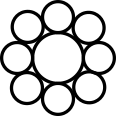
\includegraphics[width=0.5\linewidth]{figures/torons}
			\label{fig:torons}
		\end{figure}
		

	\end{minipage}
	
	
	\subsubsection{Les c\^{a}ble}
	
	
	\begin{minipage}{0.8\textwidth}
		
		Est un ensemble de torons enroulé autour d'un torons centrale.
		
	\end{minipage}
	\begin{minipage}{0.2\textwidth}
		
		\begin{figure}[H]
			\centering
			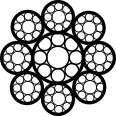
\includegraphics[width=0.7\linewidth]{figures/cables}
			\label{fig:cables}
		\end{figure}
		
		
	\end{minipage}
	
	
	
	
	
	
	
	
	
	
	
	
	
	
	
	
	
	
	
	
	
	
	
	
	
	
	
	
	
	
	
	
	
	
	
	
	
	
\end{document}